% !TeX spellcheck = pt_BR
\documentclass[12pt]{article}
\usepackage[margin=0.5in]{geometry}
\setlength{\parindent}{0pt} 
\setlength{\parskip}{5pt} 
\pagenumbering{gobble}
\setlength{\parindent}{10ex}

\usepackage[utf8]{inputenc}
\usepackage{amsmath,amsthm,amssymb}
\usepackage{graphicx}
\usepackage{float}
\usepackage[portuguese]{babel}


\title{PI IV - Visualização de dados numéricos}
\author{Lucas Gomes Santana}
\date{\today}

\begin{document}

\maketitle

\newpage
\textbf{\Large Introdução}\par
% Introdução

\newpage
\textbf{\Large Gráficos de barras empilhado}\par


\setcounter{figure}{0}
\begin{figure}[H]
\centering
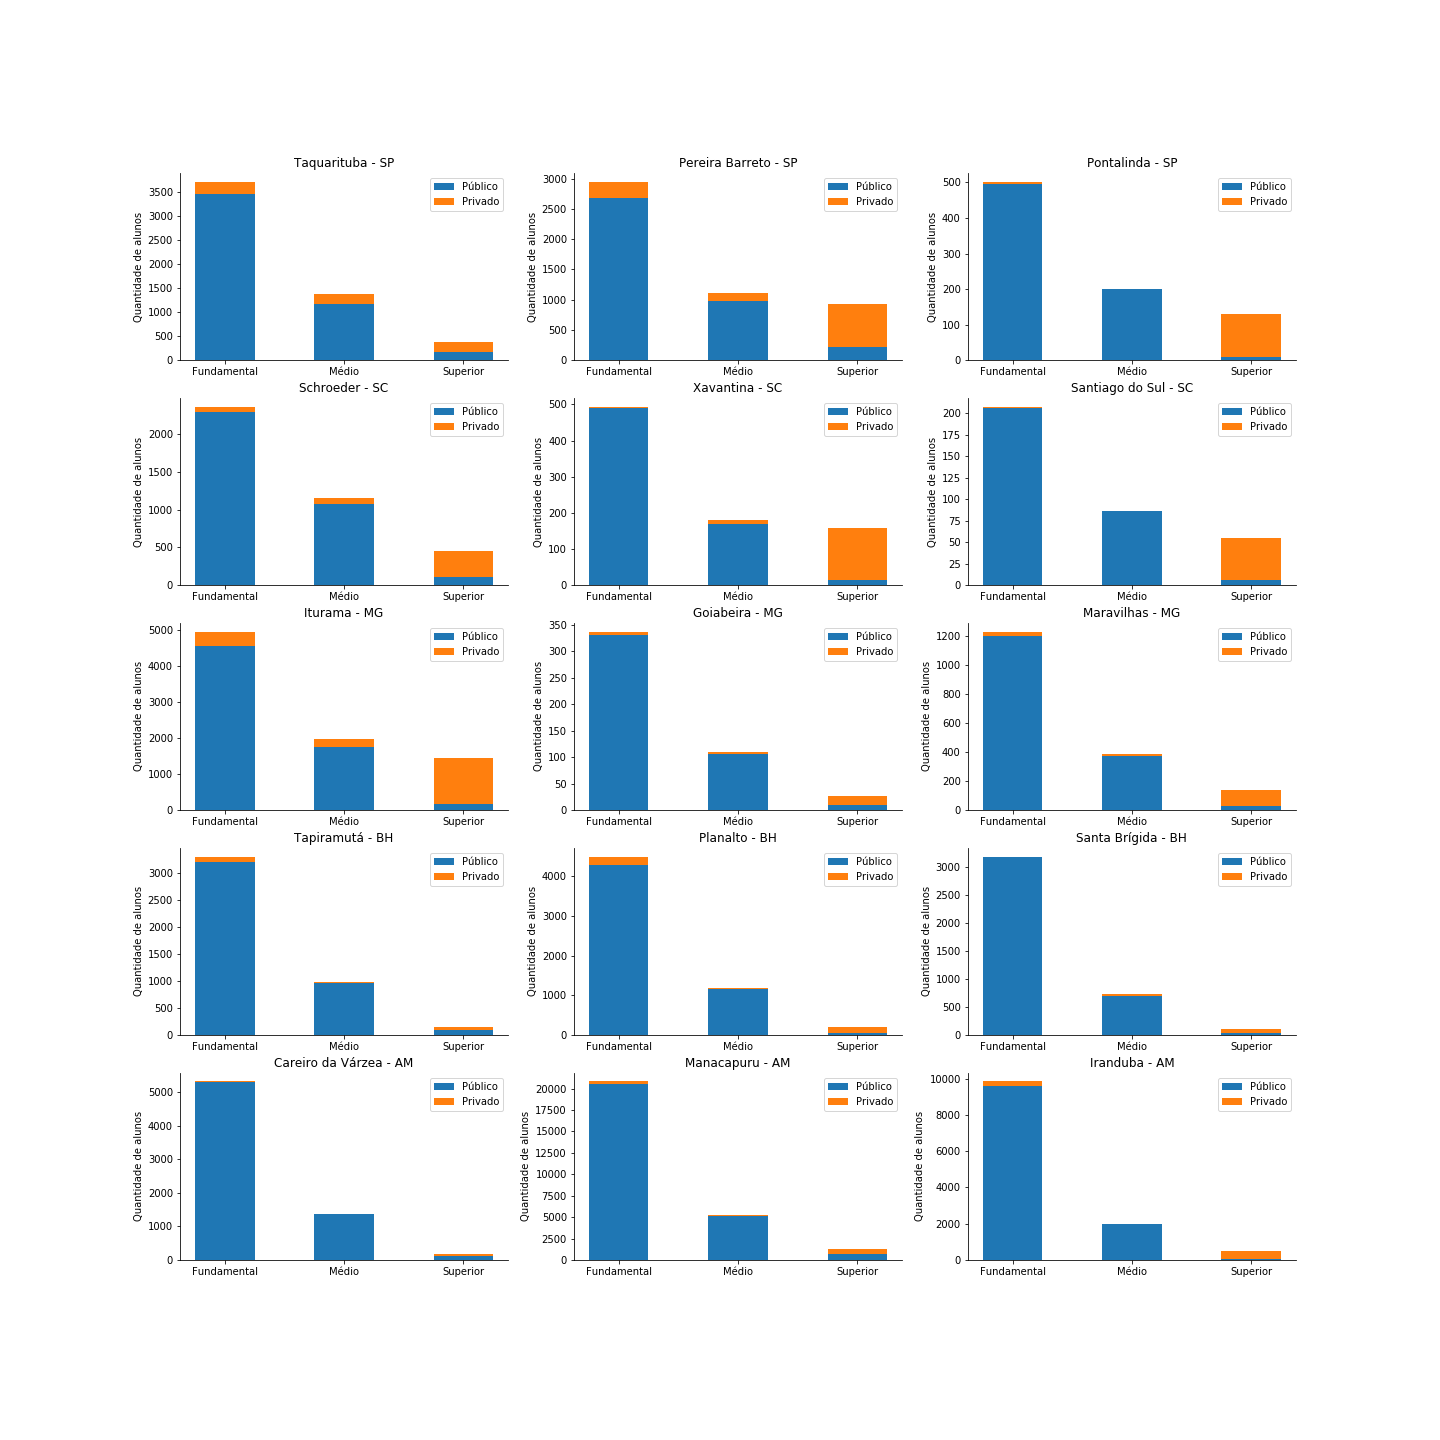
\includegraphics[width = 1\textwidth]{bar.png}
\label{fig:A.1}
\caption{Gráficos de barras mostrando o número de alunos matriculados na rede privada e pública}
\end{figure}

\newpage
\textbf{\Large Dois gráficos de pizza}\par

\setcounter{figure}{1}
\begin{figure}[H]
	\centering
	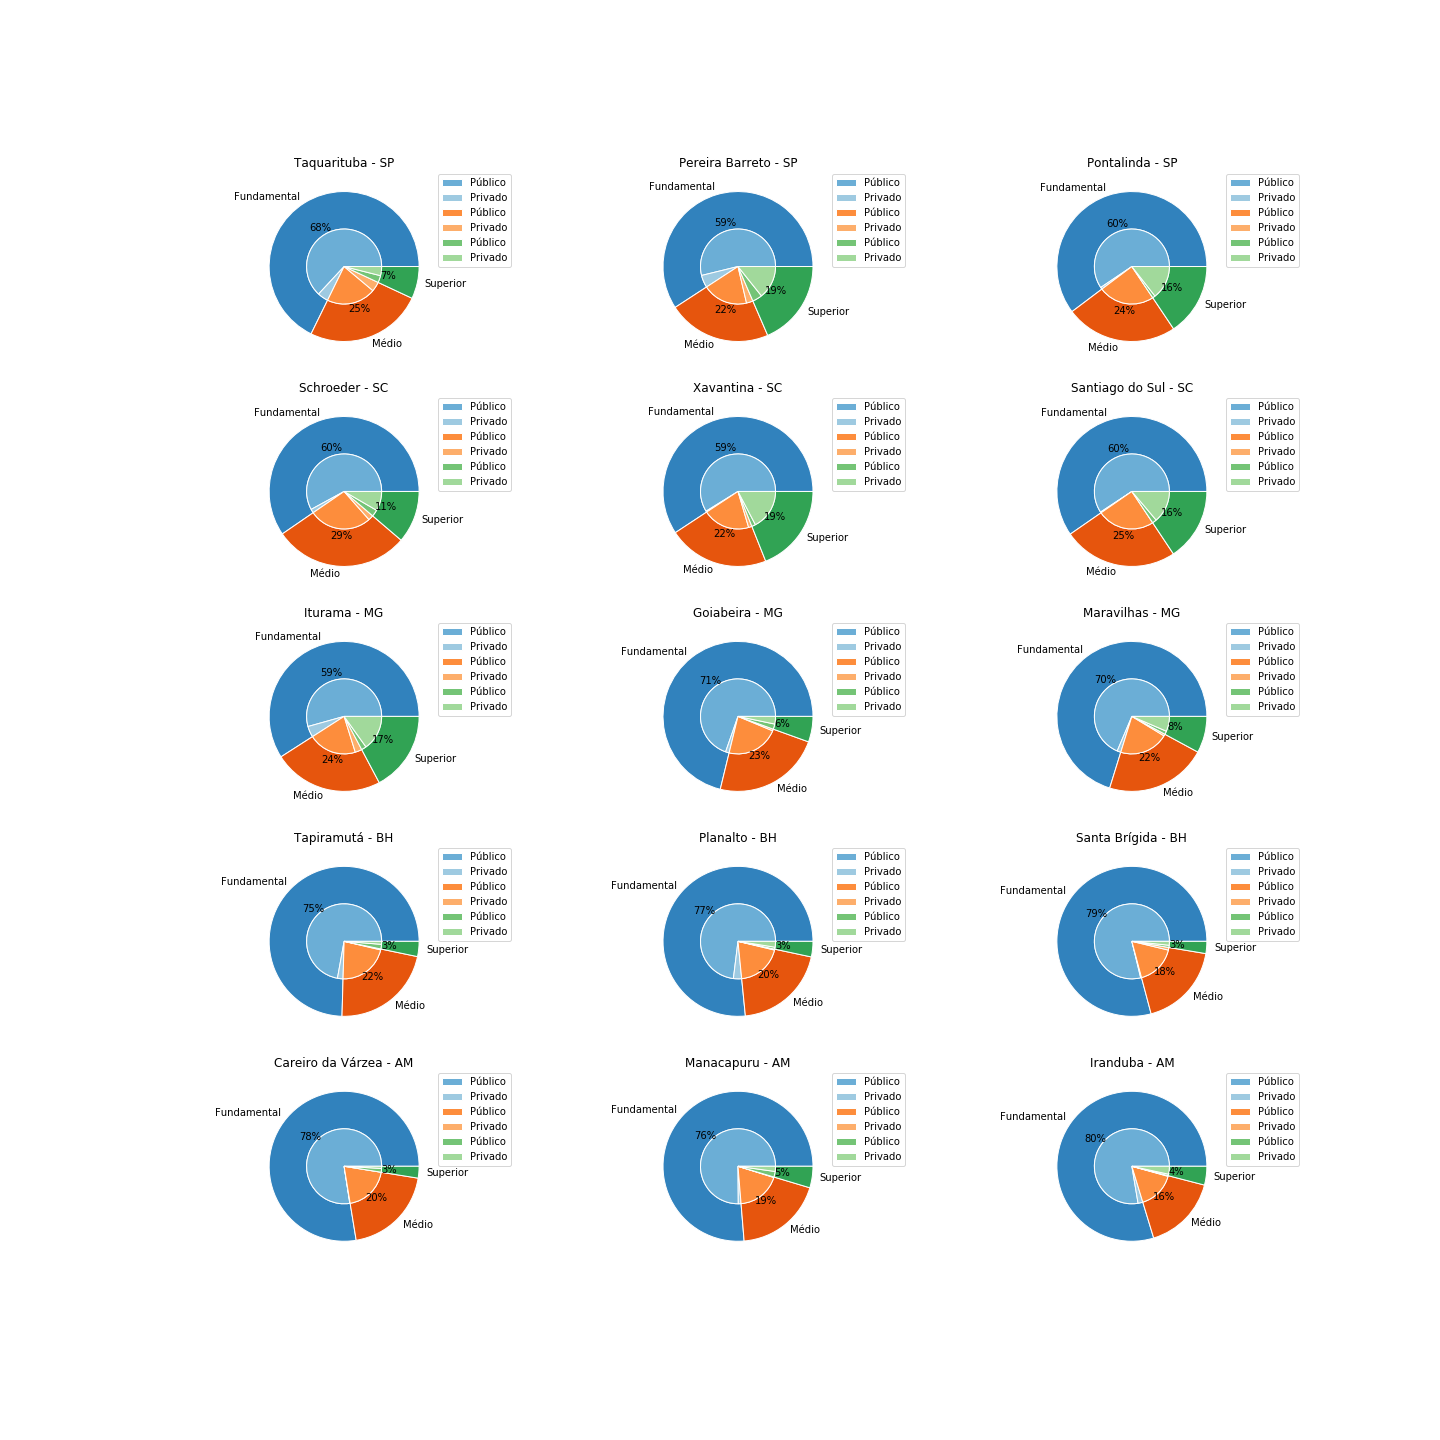
\includegraphics[width = 1\textwidth]{pie.png}
	\label{fig:A.2}
	\caption{Gráficos de pizza mostrando o número de alunos matriculados na rede privada e pública}
\end{figure}

\newpage
\textbf{\Large Comparação} \par


\newpage
\begin{thebibliography}{9}
	\bibitem{gistemp} 
	IBGE. Censo Demográfico 2010.
	Acesso em 28 de outubro de 2019. \\\texttt{https://www.ibge.gov.br/estatisticas/sociais/educacao/9662-censo-demografico-2010.html}
	
\end{thebibliography}

\end{document}